
\documentclass {article}

\setlength {\textwidth} {6in}
\setlength {\textheight} {8in}
\setlength {\topmargin} {0in}
\setlength {\oddsidemargin} {0.25in}
\setlength {\evensidemargin} {0.25in}
\addtolength {\parskip} {1ex}

\newcommand {\caps}[1] {\mbox {\ifnum\fam=0 \scshape\else\uppercase\fi{#1}}}

\newcommand {\tdadvisor} {Theses and Dissertations Advisor}
\newcommand {\csd} {Computer Science Department}
\newcommand {\regs} {{\sl Regulations for Thesis
		      and Dissertation Preparation}}
\newcommand {\ucla} {\caps {ucla}}
\newcommand {\uclacsd} {\ucla\ \csd}
\newcommand {\umi} {\caps {umi}}

\title	{ Formatting UCLA Theses and Dissertations \\
	 Using \LaTeX \\
	 and the \texttt{uclathes} Document Style}
\author {Rich Wales}
\date{}
\begin {document}
\maketitle

\newcommand{\MaintainNote}[1]{{\slshape Maintainer's note:  #1}}

\MaintainNote{
  This document was written by Rich Wales for his \texttt{thesis} style.
  I've updated it for the \texttt{uclathes} style for \LaTeX 2e.
  Typos are probably mine.
   ---John Heidemann.}


This document explains how to format your thesis%
\footnote {In order not to make this document overly verbose,
the term {\em thesis\/} will be used throughout
to indicate either a ``thesis'' (master's degree document)
or a ``dissertation'' (doctor's degree document).
The formatting requirements, in any case,
are virtually identical for both theses and dissertations.
Ph.D.\ students should understand that---%
unless indicated otherwise---%
anything said here about a {\em thesis\/}
applies with equal force to a {\em dissertation\/} as well.}
manuscript using \LaTeX.
It describes a special ``document style'' macro package
which, it is believed, will meet \ucla's requirements
regarding type size, layout, spacing, and margins.

These instructions are not intended to replace
the \ucla\ Graduate Division's publication, \regs.
All graduate students should obtain a copy of this publication,
read it carefully, and check again in advance
of the filing deadline to see if any changes have been made
to the requirements.


\section {Thesis and Dissertation Format Requirements}

Theses filed at \ucla\ are required to conform
to certain physical format specifications.
Among the reasons why such formatting issues are important
are the following:

\begin {itemize}

\item
Theses are public, published documents.
A copy of every thesis produced at \ucla\
is filed in one or more University libraries,
and are also available on microfilm
to researchers elsewhere.

Each thesis manuscript is a reflection
of the high standards of the University.
A sloppy manuscript makes the University itself look sloppy,
and so such manuscripts cannot be accepted for filing.

\item
Theses are microfilmed for archival purposes.
Additionally, doctoral dissertations are generally
microfilmed as well by University Microfilms International (\umi).
In order to ensure that the manuscript
will reproduce properly on microfilm,
it is important that the type face is sufficiently large
and that the strokes of the letters are not excessively thin.

\item
In order to guarantee successful binding
of a thesis manuscript in book form---%
as well as to ensure problem-free microfilming---%
the text margins and page number placement
must conform to known standards.

\item
Page numbering must be done in a standardized, consistent fashion,
so as to ensure that errors (such as missed pages)
will not occur in either the binding or the microfilming process.

\end {itemize}

It is crucial that a thesis manuscript
should conform to the University's formatting requirements.
A non-conforming manuscript will \emph{not} be accepted for filing---%
even if the content has been approved
by the student's committee;
even if (in the case of a problem with the signature page)
one or more committee members are not available to sign again;
and even if not enough time remains for the student
to redo the manuscript and file a satisfactory copy by the deadline.
You snooze, you loose.

In order to avoid last-minute disasters,
the \ucla\ \tdadvisor\ strongly urges \emph{all} graduate students
to submit a sample of their thesis manuscript
(including all the preliminary pages)
for review and approval well in advance of the filing deadline.
Think about how long you've been here---can't you really 
  manage to get that dissertation to Powell slightly before the
  last day to file?


\section {Using the \LaTeX\ \texttt{uclathes} Style}

This section describes how to set up
the \LaTeX\ input for your thesis
to use the \verb|uclathes| document style macros.

\subsection {Overall \LaTeX\ Source File Format}

Following are two sample \LaTeX\ input files
which illustrate the proper use of the \verb+uclathes+
document style.

Figure~\ref{fig:toplevel}
shows a ``top-level'' input file,
which itself contains only a minimal skeleton
and includes text from other files
via \verb+\input+ commands.
Figures~\ref{fig:prelim1} and \ref{fig:prelim2}
show the commands for setting up the preliminary pages.

\subsection {The $\backslash${\tt documentclass} Command}

The \verb+\documentclass+ command at the start of the \LaTeX\ input text
should have the following form:

\begin {center}
\verb+\documentclass [+{\sl options\/}\verb+] {uclathes}+
\end {center}

where {\sl options} is one of the following:

\begin {description}

\item [{\tt MS}]
--- M.S.\ thesis.

\item [{\tt PhD}]
--- Ph.D.\ dissertation.

\end {description}

Note that capitalization is important:
\verb+ms+, \verb+PHD+, or \verb+phd+ will {\em not\/} work.

The \verb+uclathes+ document style is basically the same
as the standard \LaTeX\ \verb+report+ style,
as far as the body of the text is concerned.

\subsection {The $\backslash${\tt bibliographystyle} Command}

There is a matching \verb+uclathes+ bibliography style
which should be used in conjunction with
the \verb+uclathes+ document style.
To use the \verb+uclathes+ bibliography style,
use the following \verb+\bibliographystyle+ command
near the end of your \LaTeX\ input
(just before the \verb+\end {document}+ command):

\begin {center} \verb+\bibliographystyle {uclathes}+ \end {center}

The \verb+uclathes+ bibliography style is similar to the
standard Bib\TeX\ \verb+alpha+ style.
One important new feature in the \verb+uclathes+ style is
the addition of a new \verb+annote+ field in a reference,
which can be used to produce an annotated bibliography.

\begin {figure}
{\small
\begin{verbatim}
\documentclass [PhD] {uclathes}
%%%%%%%%%%%%%%%%%%%%%%%%%%%%%%%%%%%%%%%%%%%%%%%%%%%%%%%%%%%%%%%%%%%%%%%%
%                                                                      %
%                             AKEE MACROS                              %
%                                                                      %
%%%%%%%%%%%%%%%%%%%%%%%%%%%%%%%%%%%%%%%%%%%%%%%%%%%%%%%%%%%%%%%%%%%%%%%%

\usepackage{graphicx}
\usepackage{amsmath}
\usepackage{amsfonts}
\usepackage{longtable}
\setcounter{tocdepth}{2}                         % personal LaTeX macros
%%%%%%%%%%%%%%%%%%%%%%%%%%%%%%%%%%%%%%%%%%%%%%%%%%%%%%%%%%%%%%%%%%%%%%%%
%                                                                      %
%                          PRELIMINARY PAGES                           %
%                                                                      %
%%%%%%%%%%%%%%%%%%%%%%%%%%%%%%%%%%%%%%%%%%%%%%%%%%%%%%%%%%%%%%%%%%%%%%%%

\title          {Closed-Loop Subspace Identification of a Quadrotor}
\author         {Andrew G\@. Kee}
% Note: department is really your area of research.  I.e. leave out 'Department of'.
\department     {Engineering}
% Note:  degreeyear should be optional, but as of  5-Feb-96
% it seems required or you get a year of ``2''.   -johnh
\degreeyear     {2013}

%%%%%%%%%%%%%%%%%%%%%%%%%%%%%%%%%%%%%%%%%%%%%%%%%%%%%%%%%%%%%%%%%%%%%%%%

\chair          {Steve Gibson}
%\member         {Co-chair 3 name}
%\member         {Co-chair 2 name}
%\member         {Co-chair 1 name}

%%%%%%%%%%%%%%%%%%%%%%%%%%%%%%%%%%%%%%%%%%%%%%%%%%%%%%%%%%%%%%%%%%%%%%%%

%\dedication     {\textsl{To my mother \ldots \\
%                who---among so many other things--- \\
%                saw to it that I learned to touch-type \\
%                while I was still in elementary school}}

%%%%%%%%%%%%%%%%%%%%%%%%%%%%%%%%%%%%%%%%%%%%%%%%%%%%%%%%%%%%%%%%%%%%%%%%

%\acknowledgments {(Acknowledgments omitted for brevity.)}

%%%%%%%%%%%%%%%%%%%%%%%%%%%%%%%%%%%%%%%%%%%%%%%%%%%%%%%%%%%%%%%%%%%%%%%%

\abstract {
As quadrotors begin to see widespread use in military and civilian applications, accurate dynamical system models continue to play an important role in platform development, test, and operations.  System identification provides an approach to estimating dynamical system models from system input and output data. Subspace system identification methods identify models in their state space form by exploiting the structure of the state space representation. Common subspace identification methods provide reliable results when identifying systems operating in open loop, but produce biased results when identifying systems operating in the presence of feedback (i.e.\ closed-loop systems). The Innovation Estimation Method (IEM) is a subspace identification technique that provides an approach to eliminating this bias by pre-estimating the unknown innovation sequence before carrying out subspace identification. We describe the identification of an off-the-shelf quadrotor using experimentally gathered closed-loop input-output data through subspace identification with innovation estimation. We present experimental results illustrating the ability of a model identified via IEM to accurately represent  system dynamics in the presence of feedback control.
}
%%%%%%%%%%%%%%%%%%%%%%%%%%%%%%%%%%%%%%%%%%%%%%%%%%%%%%%%%%%%%%%%%%%%%%%%

\nomenclature{

\begin{longtable}{lll}
$\mathbb{R}$ 		&& Set of all reals\\
$\mathbb{Z}$ 		&& Set of all integers\\
$A$					&& System matrix\\
$B$					&& Input matrix\\
$C$					&& Output matrix\\
$D$					&& Feedforward matrix\\
$u$					&& System input vector\\
$y$					&& System output vector\\
$e$					&& System innovation vector\\
$x$					&& System state vector\\
$v$					&& Process noise vector\\
$w$					&& Measurement noise vector\\
$n$					&& Number of system states\\
$m$					&& Number of system inputs\\
$l$					&& Number of system outputs\\
$l$					&& Number of system outputs\\
$\sigma$			&& Singular value\\
$K$					&& Kalman filter gain\\
$U_k$				&& Block Hankel matrix of system inputs\\
$U_p$				&& Block Hankel matrix of past system inputs\\
$U_f$				&& Block Hankel matrix of future system inputs\\
$Y_k$				&& Block Hankel matrix of system outputs\\
$Y_p$				&& Block Hankel matrix of past system outputs\\
$Y_f$				&& Block Hankel matrix of future system outputs\\
$X_k$				&& Block Hankel matrix of system states\\
$E_k$				&& Block Hankel matrix of system innovation\\
$E_f$				&& Block Hankel matrix of future system innovation\\
$\Gamma_k$			&& Extended observability matrix\\
$\hat{\Gamma}_f$	&& Estimate of extended observability matrix over future horizon\\
$G_f$				&& Toeplitz matrix of future Markov parameters of stochastic subsystem\\
$H_f$				&& Toeplitz matrix of future Markov parameters of deterministic subsystem\\
$f$					&& Future time horizon\\
$p$					&& Past time horizon\\
$\Pi_{U_f}^\perp$ 	&& Orthogonal projection onto the column space of $U_f$\\
$I$					&& Identity matrix\\
$Z$					&& Instrumental variable matrix\\
$Z_p$				&& Instrumental variable matrix constructed of past input-output data\\
\end{longtable}

}

%%%%%%%%%%%%%%%%%%%%%%%%%%%%%%%%%%%%%%%%%%%%%%%%%%%%%%%%%%%%%%%%%%%%%%%%
                           % preliminary page info
\begin {document}
\makeintropages
\chapter{Introduction}

Unmanned Aerial Vehicles (UAVs) have seen explosive growth in the past thirty years, performing a multitude of military and civilian tasks including surveillance, reconnaissance, armed combat operations, search and rescue, forest fire management, and domestic policing \cite{sarris2001survey, valavanis2007advances}. A class of modern UAVs which have recently grown in popularity are quadrotors -  Vertical Take Off and Landing (VTOL) vehicles powered by four rotors arranged in a cross configuration. The main advantage of the quadrotor lies in its mechanical simplicity. Adjusting the speed of one or more of the vehicle's fixed-pitch rotors provides full attitude control, eliminating the need for the swash plate mechanism found on single rotor helicopters \cite{bramwell2001bramwell, gupte2012survey}. In spite of its mechanical simplicity, the quadrotor exhibits somewhat complex dynamics that are best modeled as a Multi-Input Multi-Output (MIMO) system.

Advances in MEMS sensors and light-weight high-powered lithium polymer batteries have contributed to the recent popularity of quadrotors, making them an attractive choice for research applications in flight dynamics and control, as in \cite{hoffmann2007quadrotor, kivrak2006design, mellinger2010control, michael2010grasp}. One problem of particular interest is the development of mathematical models representing system dynamics based on experimentally gathered data. System identification provides a mechanism to relate this input-output data to the underlying system dynamics. Traditionally, system identification techniques have focused on developing a system model which minimizes prediction error. Identification methods of this form are commonly known as Prediction Error Methods (PEMs). PEMs have seen widespread use in both theoretical and real-world applications, but experience difficulties with MIMO systems as noted in \cite{qin2006overview, viberg1995subspace}. Subspace identification methods have recently grown in popularity and offer an alternative approach to the identification problem. These methods have a foundation in linear algebra and overcome the issues found in PEMs when identifying MIMO systems \cite{katayama2005subspace}. It is the goal of this research project to apply subspace identification techniques to a quadrotor using experimentally gathered closed-loop input and output data.


\section{Related Work}


\begin{figure}[htb!]
	\centering
	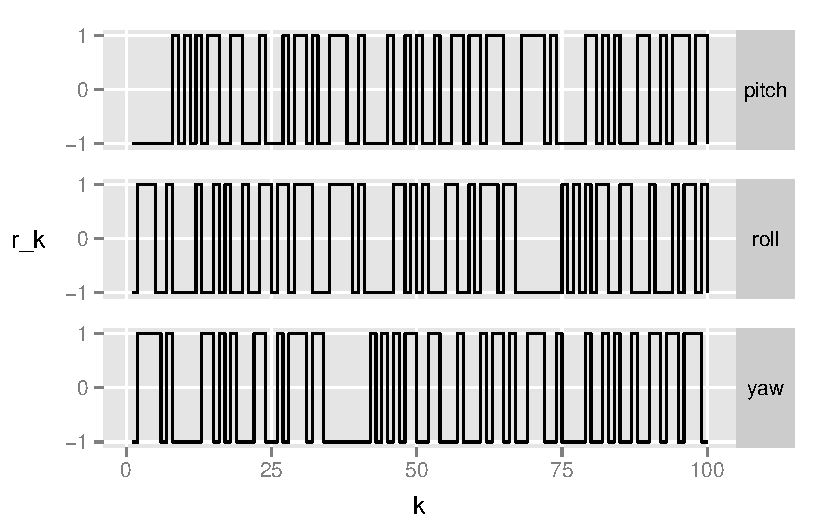
\includegraphics{../fig/prbs_input.pdf}
	\caption{A figure caption}
\end{figure}


\section{Motivation and Contributions}



                         % Chapter 1 of dissertation
\chapter{Model and Assumptions}
Introduce concept of LTI system here
\section{State Space Model}
We will consider a combined deterministic-stochastic LTI system written in innovation form as
\begin{subequations}\label{eq:2_innovation}
\begin{equation}x(k+1) = Ax(k) + Bu(k) + Ke(k)\end{equation}
\begin{equation}y(k) = Cx(k) + Du(k) + e(k)\end{equation}
\end{subequations}
where $x_k \in \mathbb{R}^n$ is the system state, $u_k \in \mathbb{R}^m$ is the system input, $y_k \in \mathbb{R}^l$ is the system output, and $e_k \in \mathbb{R}^l$ is the innovation. $A$, $B$, $C$, and $D$ are the system matrices with appropriate dimensions and $K$ is the Kalman filter gain. The system represented in (\ref{eq:2_innovation}) can also be represented in predictor form as
\begin{subequations}\label{eq:2_process}
\begin{equation}x(k+1) = A_Kx(k) + B_Ku(k) + Ky(k)\end{equation}
\begin{equation}y(k) = Cx(k) + Du(k) + e(k)\end{equation}
\end{subequations}
where $A_K = A-KC$ and $B_K = B-KD$.

The systems represented by (\ref{eq:2_innovation}) and (\ref{eq:2_process}) are equivalent from an input/output point of view, but because $A_K$ is guaranteed stable even if the original process matrix $A$ is unstable, the predictor form proves advantageous when considering unstable open-loop systems. We will use the state space model in innovation form to derive the general subspace algorithm for identifying combined deterministic-stochastic LTI systems but will rely on the prediction form of the model when considering identification of closed-loop systems.

\section{Assumptions}

\textbf{[Assumption 1]:} $A_K = A - KC$ is stable (i.e. its eigenvalues lie within the unit circle)

\noindent \textbf{[Assumption 2]:} The system is represented in its minimal form
                         % Chapter 2
\chapter{Subspace Identification Methods}
Subspace identification methods (SIM) provide an approach to identifing an unknown LTI system in its state space form using input/output data. Subspace methods rely on linear algebra techniques to extract the system matrices from the column space of the system's extended observability matrix. Considering the combined deterministic-stochastic LTI system introduced in the previous chapter, the subspace identification problem is: given a set of input and output data, estimate the system matrices $A$, $B$, $C$, and $D$ and the Kalman filter gain $K$ up to within a similarity transform. 




\subsection{Linear Algebra Tools}

\subsubsection*{Hankel Matrices}
A Hankel matrix is a matrix $H \in \mathbb{R}^{m\times n}$ with constant skew-diagonals. In other words, the value of the $(i, j)^{\mbox{th}}$ entry of $H$ depends only on the sum $i + j$.
\begin{equation*}
H_{m,n} = \begin{bmatrix}
h_1 & h_2 & \cdots & h_n\\
h_2 & h_3 & \cdots & h_{n+1}\\
\vdots & \vdots & \ddots & \vdots\\
h_m & h_{m+1} & \cdots & h_{m+n-1}
\end{bmatrix}
\end{equation*}
If each entry in the matrix is also a matrix, it is called a block Hankel matrix.


\subsubsection*{Fundamental Matrix Subspaces}
We require two of the fundamental matrix subspaces: the column space and the row space. The column space of a matrix $A \in \mathbb{R}^{m\times n}$ is the set of all linear combinations of the column vectors of $A$. The dimension of the column space is called the rank. The row space of a matrix $A \in \mathbb{R}^{m\times n}$ is the set of all linear combinations of the row vectors of $A$.


\subsubsection*{Projections}


\subsubsection*{Singular Value Decomposition}
Any matrix $A \in \mathbb{R}^{m\times n}$ can be decomposed by a singular value decomposition (SVD) given by
\begin{equation*}
A = U\Sigma V^T
\end{equation*}
where $U \in \mathbb{R}^{m\times m}$ and $V \in \mathbb{R}^{n\times n}$ are orthogonal matrices and $\Sigma \in \mathbb{R}^{m\times n}$ is diagonal matrix of the singular values of $A$ ordered such that
\begin{equation*}
\sigma_1 \geq \sigma_2 \geq \cdots \geq \sigma_k > 0
\end{equation*}




\section{Subspace Identification of Combined Deterministic-Stochastic Systems}
Considering the combined deterministic-stochastic LTI system in innovation form
\begin{subequations}
\begin{equation}x_{k+1} = Ax_k + Bu_k + Ke_k\end{equation}
\begin{equation}y_k = Cx_k + Du_k + e_k\end{equation}
\end{subequations}



A detailed derivation of this procedure follows


\section{Closed-Loop Subspace Identification}

\subsection{Identifying Systems Operating Under Feedback Control}

\subsection{Innovation Estimation Method}

\subsection{Whitening Filter}                         % etc.
\chapter{Approach}

\section{Quadrotor Platform}
Because the design and construction of a quadrotor is beyond the scope of  this project, we will use a commercially available vehicle called the Bitcraze Crazyflie \cite{bitcraze}. The Crazyflie, shown in Figure \ref{fig:quad} is a small, low cost, open-source quadrotor kit suitable for indoor flight. It measures 9 cm motor to motor and weighs 19 grams. A 170 mAh lithium-polymer battery powers the vehicle, providing 7 minutes of flight time. An onboard microcontroller is responsible for vehicle stabilization and control and reads sensor measurements from a three-axis accelerometer, three-axis gyroscope, three-axis magnetometer, and barometer.
\begin{figure}[!htb]
\centering 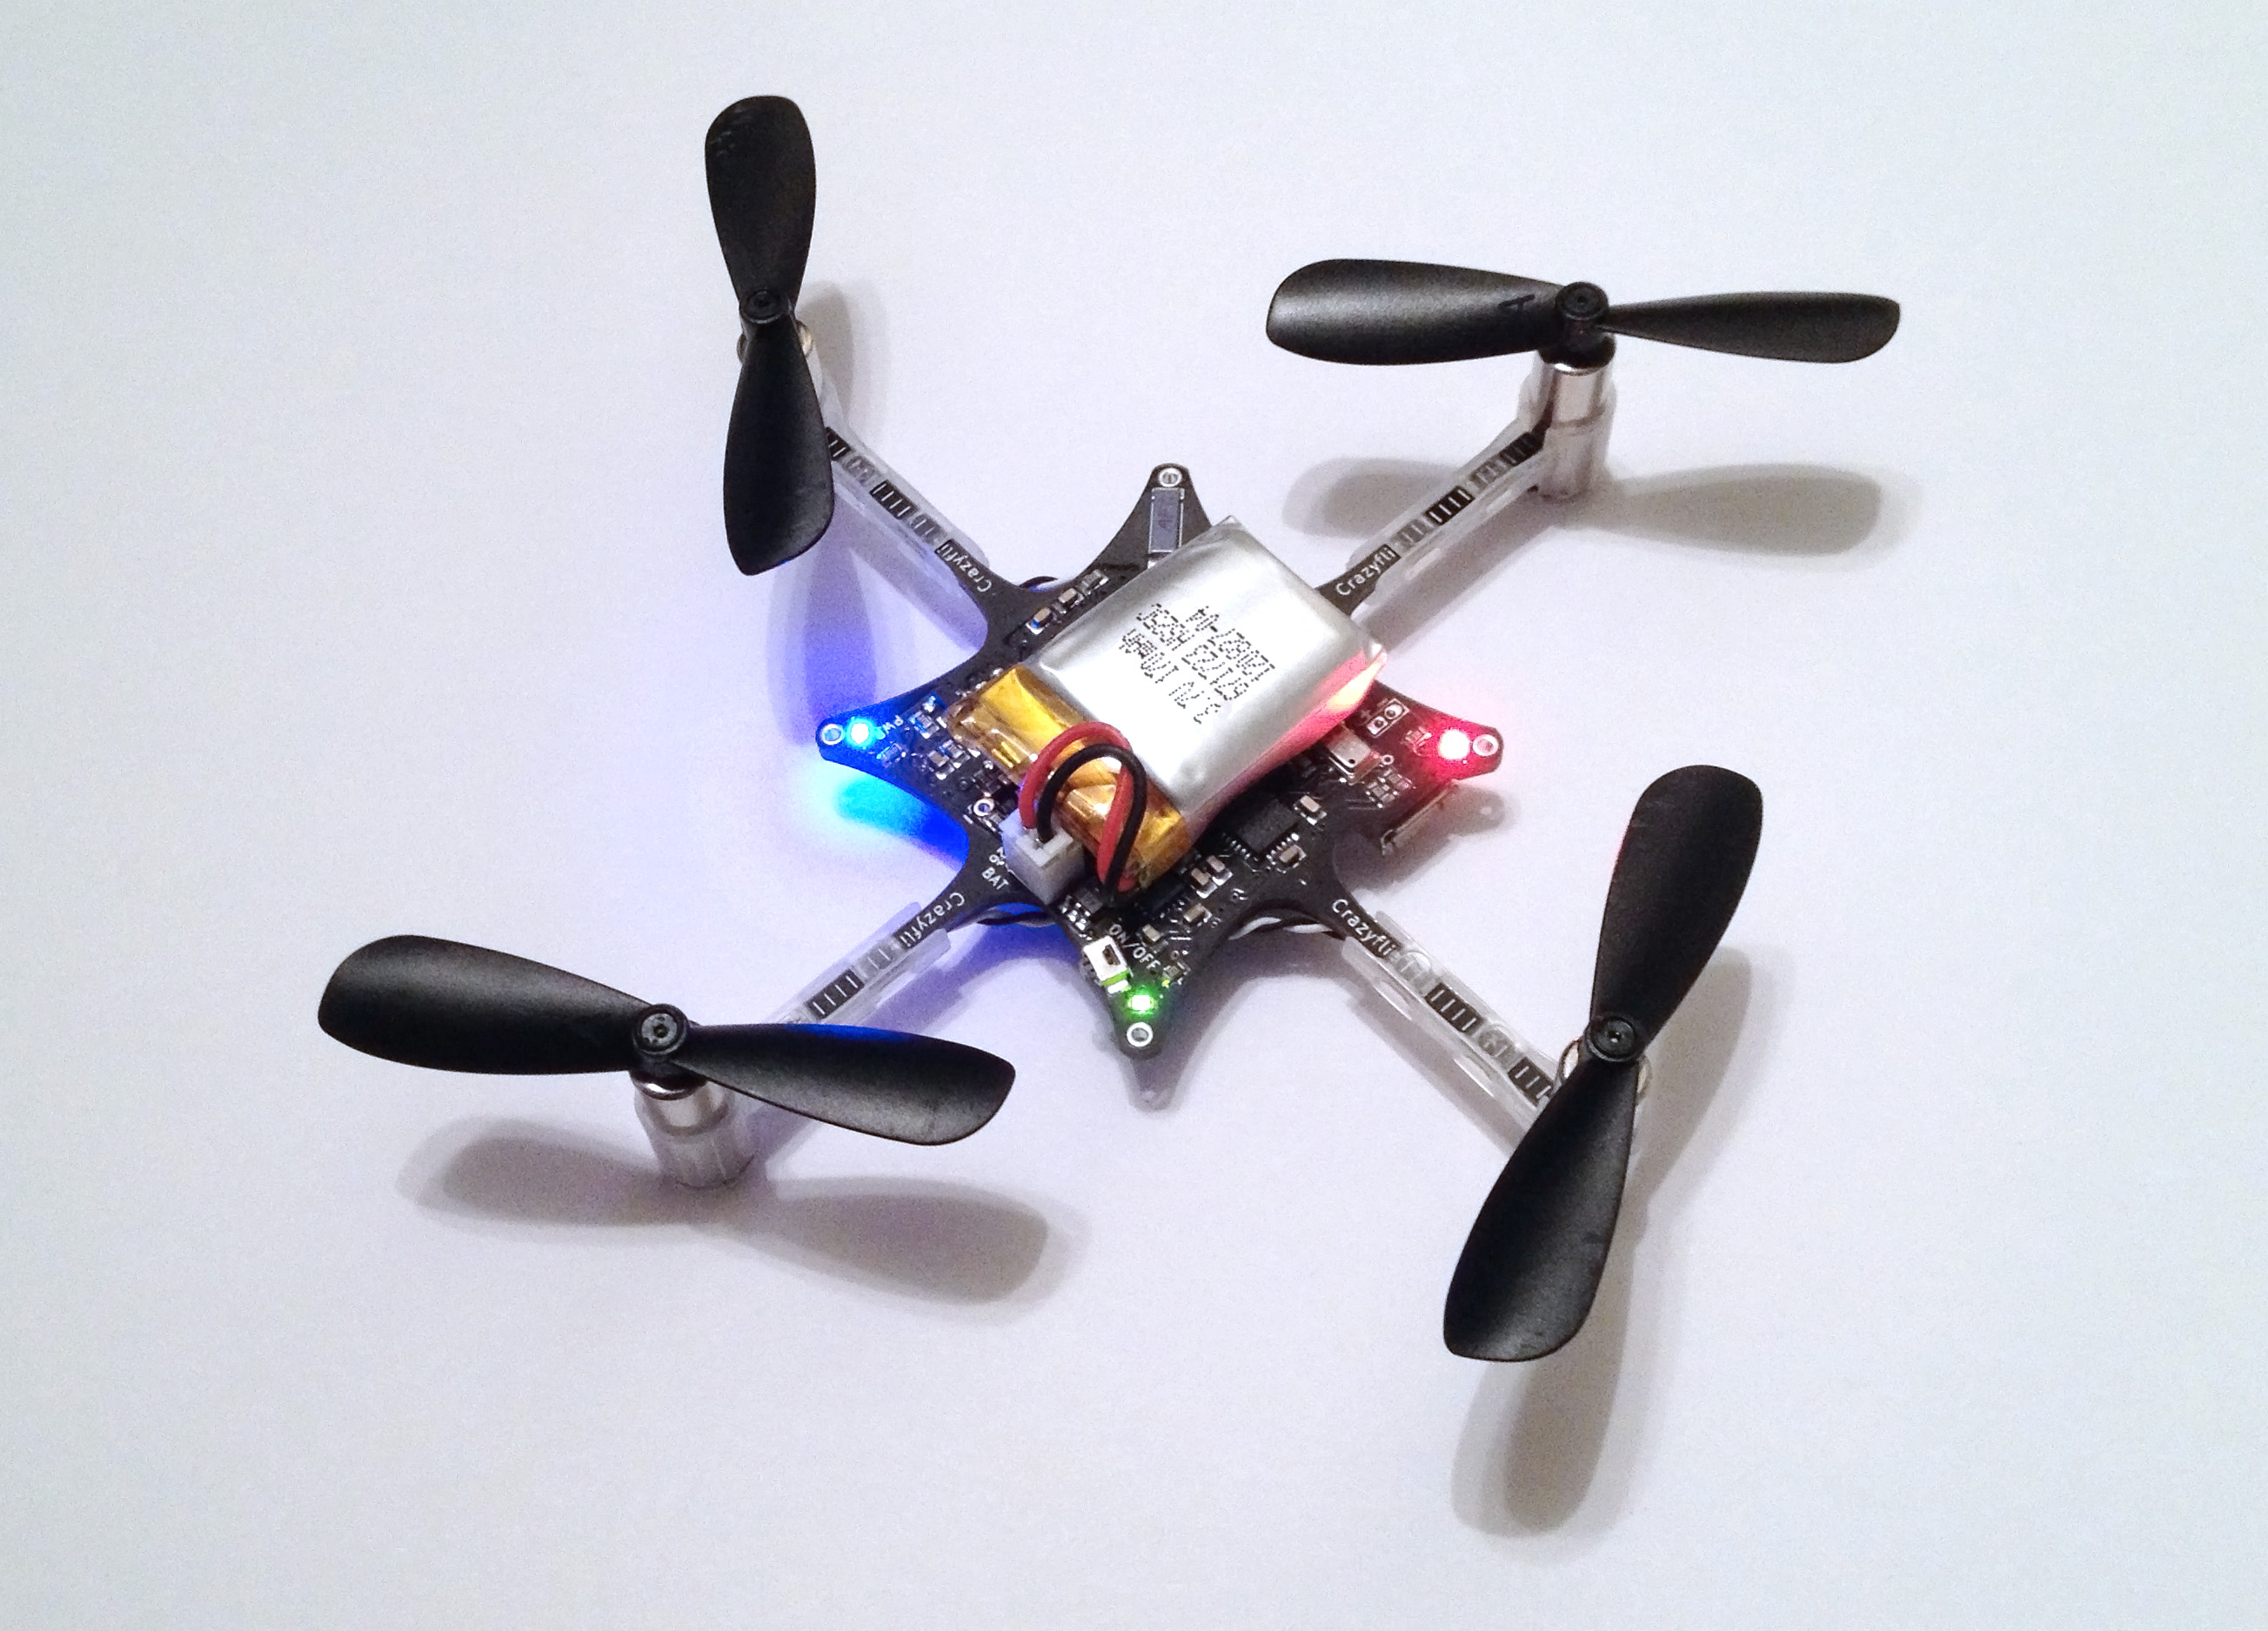
\includegraphics[scale=.15]{../fig/crazyflie.jpg}
\caption{Bitcraze Crazyflie Quadrotor}
\label{fig:quad}
\end{figure}

Vehicle pitch, roll, yaw, and thrust inputs are set in one of two ways. First, a USB gamepad connected to a computer running the Crazyflie PC client provides a method for direct user control of the vehicle. Second, the PC client exposes a Python API, making it possible to programmatically send the vehicle control set-points. The vehicle receives control inputs and transmits telemetry data wirelessly over a 2.4 GHz radio connection to a USB radio dongle connected to the Crazyflie PC client running on a laptop computer.
\begin{figure}[htb!]
	\centering
	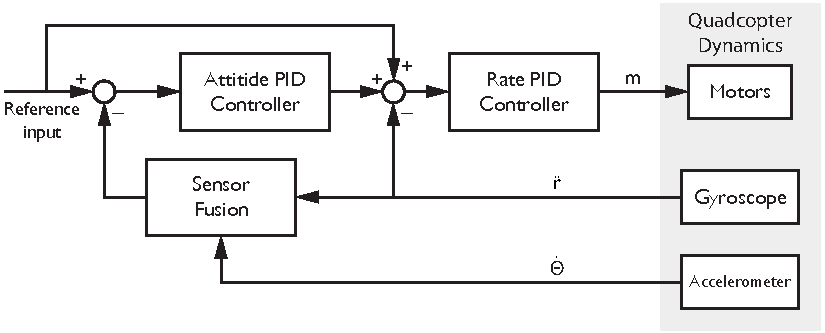
\includegraphics{../fig/crazyflie_control_system_block_diagram.pdf}
	\caption{Crazyflie control system block diagram}
\end{figure}

\section{Experiment Design}
blah

\section{Data Collection}



\section{Data Analysis}
INCLUDE OVERVIEW OF WFA ALGORITHM IN BOX (MATH-BASED) IN THIS SECTION


\section{Verification}
\chapter{Closed-Loop Subspace Identification of a Quadrotor}\label{results}
\section{Identification Results}
Using closed-loop input-output data captured from test flights of a quadrotor operating under PRBS inputs, we developed an LTI system model using subspace identification techniques with innovation estimation following the procedure outlined in Chapter \ref{approach}.

\subsection{Experimental Data Used for Identification}
We conducted many test flights and ultimately identified 18 data sequences of high enough quality to use for model identification and verification. Of these sequences, nine were collected with the vehicle operating under PRBS inputs and nine were collected with the vehicle operating under individual DOF excitation inputs (three each for pitch, roll, and yaw). While we considered concatenating multiple data sequences together into a longer single input-output sequence, models identified with an individual sequence proved to adequately capture desired system dynamics.


\subsection{Model Order Selection}
System order selection occurs as a part of the model identification procedure. A plot of the singular values of the extended observability matrix, shown in Figure \ref{singular_values} is intended to provide a visual means to select the best system order. 
\begin{figure}[b!]
	\centering
	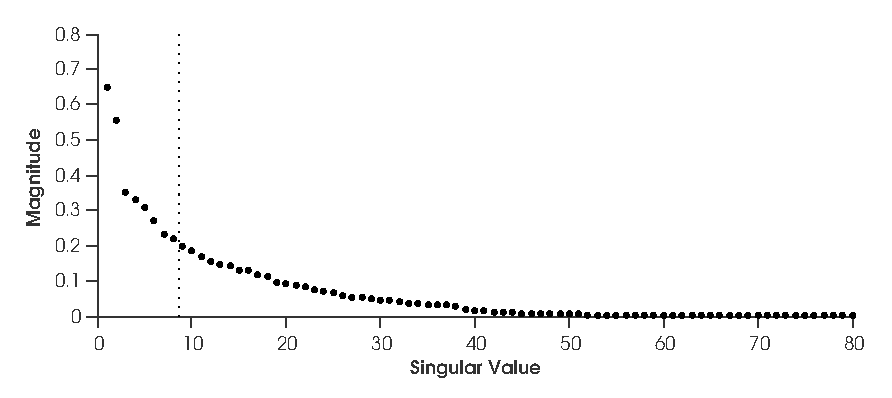
\includegraphics{../fig/singular_values_parsim.eps}
	\caption{A plot of the singular values of the extended observability matrix, used to determine the model order. The vertical dotted line shows the partitioning location between system response and noise in the final eighth order model.}
	\label{singular_values}
\end{figure}
From the figure, we see a significant drop in the magnitude of the singular values after the second, but selecting a system order of two did not adequately model the system dynamics. As a result, we tested a number of models with orders ranging from 3 to 12 and ultimately selected an 8th order model because it consistently produced reliable results from multiple PRBS data sets.

\subsection{Past and Future Horizon for Innovation Estimation}
Estimation of the innovation sequence requires the definition of past and future estimation horizons. We experimentally determined past and future horizon values by identifying a number of system models by varying the past and future horizons, first in coarse increments and later in finer increments. By evaluating the performance of a set of models identified over a range of coarsely spaced horizons, we were able to narrow the time horizon window and evaluate a smaller set of models identified  over a range of finely spaced horizons, eventually settling on the best model. For the final system model, we used a past estimation horizon of 60 and a future estimation horizon of 17. 

By plotting the poles of all evaluated models (Figure \ref{fig:poles_all}), we see the most common pole locations. The poles of the final system model, plotted in Figure \ref{fig:poles_1760} show the model is stable and only one pole has an oscillatory response (the pole is located in the left half of the real plane). This is in contrast to the full set of models, which most commonly have three poles exhibiting an oscillatory response. The single oscillatory pole in the final system model is also faster than each of the three poles common to the set of all models, which increases the overall responsiveness of the final model. 

\begin{figure}[htb!]
	\centering
	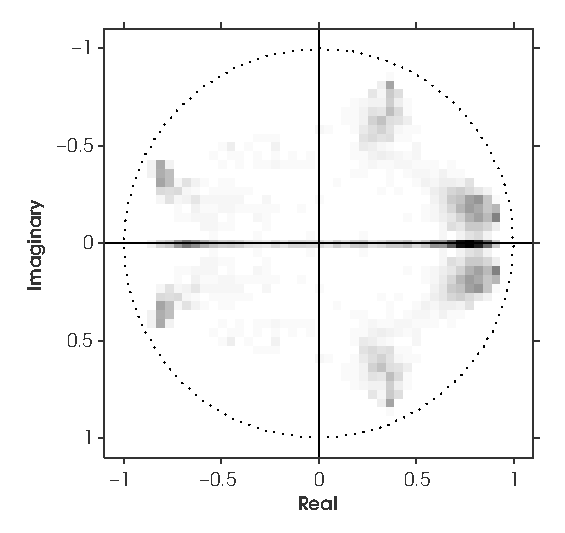
\includegraphics{../fig/poles_all.eps}
	\caption{Pole distribution of 8th order models generated for 756 combinations of past and future horizons. Darker shading indicates higher pole concentrations.}
	\label{fig:poles_all}
\end{figure}

\begin{figure}[htb!]
	\centering
	\includegraphics{../fig/poles_1760.eps}
	\caption{Poles of final 8th order model.}
	\label{fig:poles_1760}
\end{figure}


\subsection{Identified 6DOF Quadcopter Model}
The final 8th order quadrotor LTI model identified using innovation estimation, given in its state space form is 
\begin{subequations}\label{eq:2_lti}
\begin{equation*}x(k+1) = Ax(k) + Bu(k)\end{equation*}
\begin{equation*}y(k) = Cx(k) + Du(k)\end{equation*}
\end{subequations}
where system input $u = \begin{bmatrix}u_1 & u_2 & u_3 & u_4\end{bmatrix}^T$ is a vector of motor commands and system output $y = \begin{bmatrix}\ddot x & \ddot y & \ddot z & p & q & r\end{bmatrix}^T$ is a vector of accelerometer and gyroscope measurements. The system matrices of the model appear fully in Table \ref{identified_system_matrices}.

\begin{table}[!htb]
\centering
\caption{Identified System Matrices, 8th order LTI Quadrotor Model}%\vspace{0.5em}
\fbox{
\begin{minipage}{5.5in}
\footnotesize % DECREASE FONT SIZE
\begin{equation*}
A = \begin{bmatrix}
0.8521&-0.0304&-0.2107&0.3639&0.0859&-0.2501&0.0172&-0.0448\\
-0.0794&0.7874&0.1238&0.2699&0.4075&0.0408&-0.3177&-0.0088\\
0.1025&-0.0053&0.5120&-0.4573&0.3561&-0.5139&0.0986&-0.1669\\
-0.0379&0.0325&-0.5483&-0.3013&0.4049&-0.0075&0.1634&0.3805\\
0.0042&-0.0926&0.0224&0.1017&0.5170&0.3392&0.5775&-0.2288\\
0.1567&-0.0832&0.5616&0.2255&-0.0186&0.3945&0.2078&0.4095\\
0.0077&0.0579&0.0469&0.0398&-0.0686&-0.2426&-0.0026&0.2523\\
-0.0622&0.0535&-0.0811&0.0428&0.1020&-0.0254&0.0795&0.4353
\end{bmatrix}
\end{equation*}
\begin{equation*}
B = \begin{bmatrix}
-0.0025&-0.0037&-0.0112&-0.0017\\
0.0022&0.0027&0.0039&0.0045\\
-0.0038&-0.0018&0.0101&-0.0024\\
0.0098&0.0090&-0.0020&0.0037\\
-0.0011&0.0063&-0.0035&0.0027\\
0.0077&0.0107&0.0038&0.0054\\
-0.0009&-0.0085&-0.0032&-0.0058\\
-0.0013&-0.0042&-0.0072&-0.0047
\end{bmatrix}
\end{equation*}   
\begin{equation*}
C = \begin{bmatrix}
-0.0001&0&-0.0001&0.0001&-0.0001&0.0002&0.0003&-0.0003\\
0&0&0.0001&-0.0001&0.0002&-0.0001&-0.0002&0.0003\\
0.0001&-0.0001&0&0&-0.0002&0.0003&0.0000&-0.0004\\
-0.0252&-0.5396&0.0367&0.0661&0.4731&0.1647&-0.6491&0.0088\\
-0.4569&-0.2298&-0.0069&0.6147&0.1088&-0.5000&0.1831&0.0206\\
-0.0116&0.0591&0.0035&0.0091&0.0085&-0.0450&0.0297&-0.0022
\end{bmatrix}
\end{equation*} 
\begin{equation*}
D = \begin{bmatrix}
0&0&0&0\\
0&0&0&0\\
0&0&0&0\\
0&0&0&0\\
0&0&0&0\\
0&0&0&0
\end{bmatrix}
\end{equation*}
\normalsize % INCREASE FONT SIZE
\end{minipage}}
\label{identified_system_matrices}
\end{table}



%Stimulating the system with a step response provides insight into the model performance (Figure \ref{fig:5_step}).
%\begin{figure}[htb!]\label{fig:5_step}
%	\centering
%	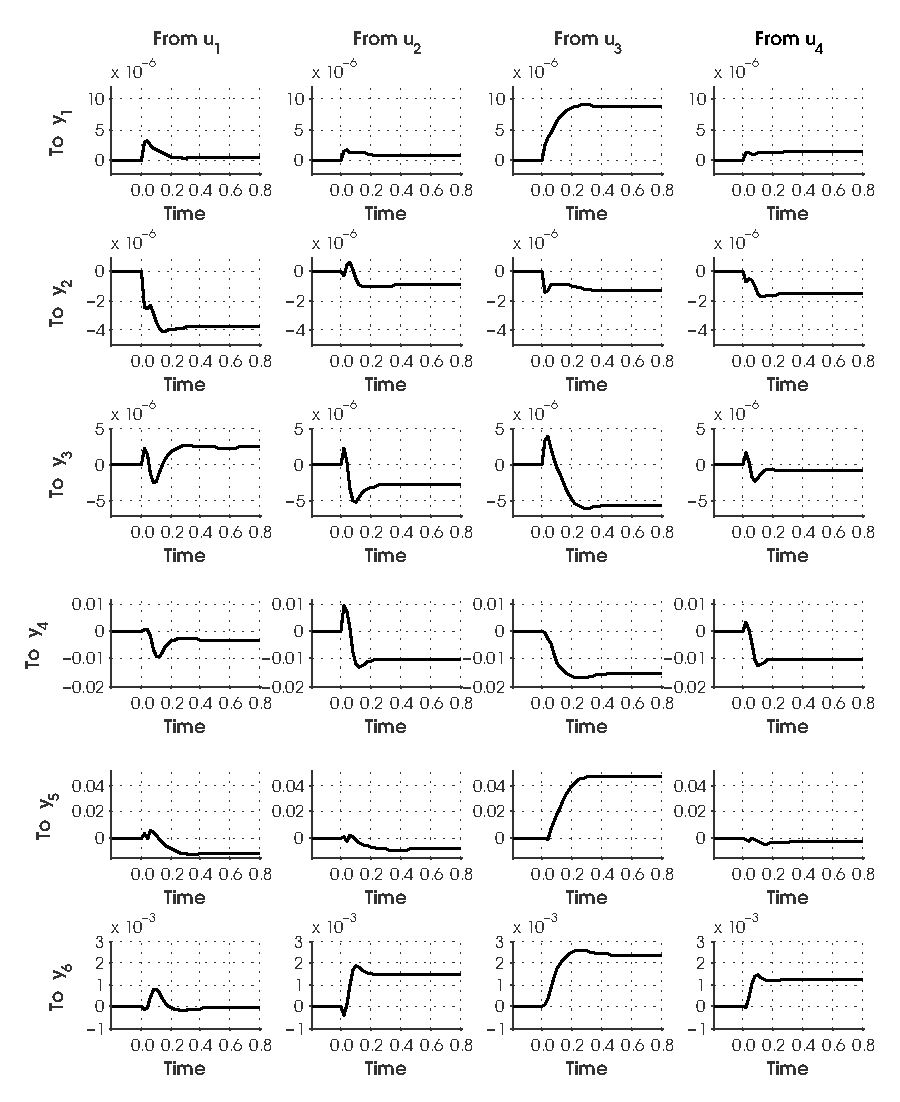
\includegraphics{../fig/step_resp_parsim.eps}
%	\caption{Step response of the 8th order system model.}
%\end{figure}\clearpage






\newpage
\section{Time Domain Model Validation}
Comparing system response predicted by the identified model with measured system response originating from the same input sequence provides a straightforward way to validate the identified model in the time domain. We compared the identified model's time domain response with the measured response of the physical system using four different input sequences: PRBS input, pure pitch input, pure roll input, and pure yaw input. 

Because the IEM deals with the coupling between system input and past noise present in a closed-loop system by pre-estimating the noise sequence from the input-output data used for identification, some real system dynamics are inevitably ``estimated out'' of the model during this procedure. This is evident in the fact that some of the faster system modes are not perfectly represented.

By evaluating the identified model's ability to represent the decoupled dynamics of the physical system, we are able to draw conclusions about the ability of a PRBS input sequence to identify individual dynamical modes of a system. During the pure pitch, roll, and yaw input sequences, the non-excited degrees of freedom were not fixed and thus the vehicle was free to move in all six degrees of freedom.

\subsection{Evaluation of Full 6DOF LTI Model Dynamics}
Figure \ref{sim_1760_20131017212626_31_38500} shows the comparison of system response between the identified model and the physical system. In general, the identified model provides a satisfactory estimate of the physical system dynamics. The pitch and roll rates are accurately predicted and the magnitudes of the $x$, $y$, and $z$ accelerations are correctly predicted. 

While the system acceleration predictions are accurate with respect to the magnitude of acceleration, it is not surprising that the predictions do not more closely follow the measured response. This is due to the fact that the accelerometers are very susceptible to measuring vehicle vibrations caused by slightly unbalanced motors and propellers. Because these vibrations occur at a much higher frequency than the Nyquist frequency, they are not captured by the identified model and thus not reflected in the system response.

Inspecting the yaw rate response, we see that the model does not accurately capture the yaw dynamics of the physical system. We observed this deficiency in all verification tests when comparing simulated model response with the measured response of the physical system. We hypothesize that this failure to successfully identify the yaw dynamics is due to the way a quadrotor's yaw mode is excited. While the pitch and roll modes of a quadrotor are excited by changing the rotor speed of only two opposing rotors, excitation of the yaw mode requires speed changes to all four rotors. It is possible that a higher order system model would capture these dynamics, although we tested models up to 12th order without success. This problem is not isolated; others including \cite{lee2011attitude} and \cite{mettler2000system} have experienced similar difficulties identifying yaw dynamics in rotorcraft.

\subsection{Evaluation of LTI Model Pitch Dynamics}
Figure \ref{sim_1760_pitch} shows the comparison of system response between the identified model and the physical system excited by pure pitch inputs. The simulated pitch rate aligns with the measured value showing that the model accurately represents isolated pitch dynamics of the system.


\subsection{Evaluation of LTI Model Roll Dynamics}
Figure \ref{sim_1760_roll} shows the comparison of system response between the identified model and the physical system excited by pure roll inputs. The simulated roll rate generally tracks the measured value. In several places, the measured roll rate is clipped while the predicted value is not clipped (in particular between 1.5 and 2 seconds). This is likely due to nonlinearities in the physical system not captured by the linear model.


\subsection{Evaluation of LTI Model Yaw Dynamics}
Figure \ref{sim_1760_yaw} shows the comparison of system response between the identified model and the physical system excited by pure yaw inputs. The identified model does not accurately capture the isolated yaw dynamics of the physical system. This is expected, as the model also failed to adequately represent the yaw dynamics of the full 6DOF system operating under PRBS input. Inspection of the pitch and roll rate responses in Figure \ref{sim_1760_yaw} reveals a coupling between yaw input and simulated pitch and roll rate. Both yaw inputs beginning at 1.7 seconds and 2.2 seconds result in responses in simulated pitch and roll rates. This effect is not seen in the physical system. The yaw dynamics are not completely missed however. From Figure \label{sim_1760_20131017212626_31_38500} we see that after 2 seconds, the simulated response somewhat tracks the measured output for small angle changes.







\newpage
\begin{figure}[htb!]
	\centering
	\includegraphics{../fig/sim_1760_20131017212626_31_38500.eps}
	\caption{Simulated response (dashed) of identified 8th order LTI system model compared with measured system response (solid). Both systems were stimulated with an identical PRBS input sequence.}
	\label{sim_1760_20131017212626_31_38500}
\end{figure}\clearpage

\newpage
\begin{figure}[htb!]
	\centering
	\includegraphics{../fig/sim_1760_pitch.eps}
	\caption{Simulated (dashed) response of identified model to pitch input compared with measured system response (solid).}
	\label{sim_1760_pitch}
\end{figure}\clearpage

\newpage
\begin{figure}[htb!]
	\centering
	\includegraphics{../fig/sim_1760_roll.eps}
	\caption{Simulated (dashed) response of identified model to roll input compared with measured system response (solid).}
	\label{sim_1760_roll}
\end{figure}\clearpage

\newpage
\begin{figure}[htb!]
	\centering
	\includegraphics{../fig/sim_1760_yaw.eps}
	\caption{Simulated (dashed) response of identified model to yaw input compared with measured system response (solid).}
	\label{sim_1760_yaw}
\end{figure}\clearpage


\newpage
\section{Comparing Identified Model Performance From PO-MOESP and IEM Algorithms With Closed-Loop Data}
In addition to evaluating the performance of a model identified using a closed loop subspace identification method (IEM), we analyzed the performance of a model identified from the same closed-loop data using a traditional subspace identification method which makes no attempt to correct  (PO-MOESP). Because we used the same input-output data to develop both models, the only differences between the two models are due to the identification algorithms used. 

Unlike IEM, the PO-MOESP algorithm assumes no correlation between system input an past noise (an invalid assumption in this case), with the effect of violating this assumption is easily seen in Figure \ref{sim_1760_moesp.eps}. Because PO-MOESP makes no attempt to deal with the coupling between the input and noise terms however, the model identified using PO-MOESP does not suffer from the issue of having true system dynamics pre-estimated out. The result is that although the magnitudes of estimated system responses are incorrect, the model identified using PO-MOESP tracks the true system better than the IEM model in some cases. Despite this fact, the IEM model provides a more correct representation of the overall dynamics of the physical system in the presence of closed-loop data.

\newpage
\begin{figure}[htb!]
	\centering
	\includegraphics{../fig/sim_1760_moesp.eps}
	\caption{Simulated (dashed) response of identified model to yaw input compared with measured system response (solid). IEM results are plotted in light gray (solid) for reference.}
	\label{sim_1760_moesp.eps}
\end{figure}\clearpage












\chapter{Conclusion}


\subsection{Conclusion}



\section{Future Work}
\input {chapter7}
\input {chapter8}
\bibliography {bib/network,bib/naming}    % bibliography references
\bibliographystyle {uclathes}
\end {document}
\end{verbatim}
}
\caption {Top-Level \LaTeX\ Input File ({\tt diss.tex})}
\label {fig:toplevel}
\end {figure}
\begin {figure}
{\small
\begin{verbatim}
%%%%%%%%%%%%%%%%%%%%%%%%%%%%%%%%%%%%%%%%%%%%%%%%%%%%%%%%%%%%%%%%%%%%%%%%
%                                                                      %
%                          PRELIMINARY PAGES                           %
%                                                                      %
%%%%%%%%%%%%%%%%%%%%%%%%%%%%%%%%%%%%%%%%%%%%%%%%%%%%%%%%%%%%%%%%%%%%%%%%

\title          {Improving the Throughput \\
                of Connectionless Datagram Protocols \\
                over Networks with Limited Bandwidth}
\author         {Richard Bert Wales}
\department     {Computer Science}

%%%%%%%%%%%%%%%%%%%%%%%%%%%%%%%%%%%%%%%%%%%%%%%%%%%%%%%%%%%%%%%%%%%%%%%%

\chair          {Jack W.\ Carlyle}
\member         {Mario Gerla}
\member         {David G.\ Cantor}
\member         {Richard L.\ Baker}
\member         {Robert M.\ Stevenson}

%%%%%%%%%%%%%%%%%%%%%%%%%%%%%%%%%%%%%%%%%%%%%%%%%%%%%%%%%%%%%%%%%%%%%%%%

\dedication     {\sl To my mother \ldots \\
                who---among so many other things--- \\
                saw to it that I learned to touch-type \\
                while I was still in elementary school}

%%%%%%%%%%%%%%%%%%%%%%%%%%%%%%%%%%%%%%%%%%%%%%%%%%%%%%%%%%%%%%%%%%%%%%%%

\acknowledgments {(Acknowledgments omitted for brevity)}

%%%%%%%%%%%%%%%%%%%%%%%%%%%%%%%%%%%%%%%%%%%%%%%%%%%%%%%%%%%%%%%%%%%%%%%%

\vitaitem   {1952}
                {Born, San Francisco, California, USA.}
\vitaitem   {1974--1975}
                {Campus computer center ``User Services'' programmer and
                consultant, Stanford Center for Information Processing,
                Stanford University, Stanford, California.}
\end{verbatim}
}
\caption {Preliminary Page Info ({\tt prelim.tex})---Part 1 of 2}
\label {fig:prelim1}
\end {figure}

\begin {figure}
{\small
\begin{verbatim}
\vitaitem   {1974--1975}
                {Programmer, Housing Office, Stanford University.
                Designed a major software system for assigning
                students to on-campus housing.
                With some later improvements, it is still in use.}
\vitaitem   {1975}
                {B.S.~(Mathematics) and A.B.~(Music),
                Stanford University.}
\vitaitem   {1977}
                {M.A.~(Music), UCLA, Los Angeles, California.}
\vitaitem   {1977--1979}
                {Teaching Assistant, Computer Science Department, UCLA.
                Taught sections of Engineering 10 (beginning computer
                programming course) under direction of Professor Leon
                Levine.
                During summer 1979, taught a beginning programming
                course as part of the Freshman Summer Program.}
\vitaitem   {1979}
                {M.S.~(Computer Science), UCLA.}
\vitaitem   {1979--1980}
                {Teaching Assistant, Computer Science Department, UCLA.}
\vitaitem   {1980--1981}
                {Research Assistant, Computer Science Department, UCLA.}
\vitaitem   {1981--present}
                {Programmer/Analyst, Computer Science Department, UCLA.}

%%%%%%%%%%%%%%%%%%%%%%%%%%%%%%%%%%%%%%%%%%%%%%%%%%%%%%%%%%%%%%%%%%%%%%%%

\publication    {{\sl MADHOUS Reference Manual.}
                Stanford University, Dean of Student Affairs
                (Residential Education Division), 1978.
                Technical documentation for the MADHOUS
                software system used to assign students to
                on-campus housing.}

%%%%%%%%%%%%%%%%%%%%%%%%%%%%%%%%%%%%%%%%%%%%%%%%%%%%%%%%%%%%%%%%%%%%%%%%

\abstract       {(Abstract omitted for brevity)}

%%%%%%%%%%%%%%%%%%%%%%%%%%%%%%%%%%%%%%%%%%%%%%%%%%%%%%%%%%%%%%%%%%%%%%%%
\end{verbatim}
}

\caption {Preliminary Page Info ({\tt prelim.tex})---Part 2 of 2}
\label {fig:prelim2}
\end {figure}

\section {Commands for Preliminary Pages}

In order to ensure that the preliminary pages
of the thesis are in the proper format,
the \verb+uclathes+ document style macros
include all the instructions necessary
to produce these pages.
All you, the student, need to do
is to specify the various pieces of information
(names, titles, etc.)
in a series of special commands as described below.
These commands should be placed at the very beginning
of the \LaTeX\ input---%
{\em before\/} the \verb+\begin {document}+ command.
The very first command
after the \verb+\begin {document}+ command
should be the \verb+\makeintropages+ command already described.

Although it is by no means mandatory,
it is strongly recommended
that you put all of the following ``declaration'' commands
pertaining to the preliminary pages
into a separate source file
(possibly with a file name like \verb+prelim.tex+
or \verb+chapter0.tex+),
and then refer to this file via an \verb+\input+ command
in your main source file.

Note that those headings on preliminary pages
which are shown in FULL CAPITALS in \regs\
are produced in {\sc Upper/Lower Small Capitals}
by the \verb+uclathes+ document style.
Also, the thesis title---%
as well as the student's name on the title page---%
will appear in large, bold type.
The last time I checked,
the \tdadvisor\ had approved these variations.%
\footnote {See the section
``If the Dissertation Advisor Gives You Trouble''
before you go to file your manuscript.}

\subsection {Title Page Information}

The title of your thesis should be specified
via a \verb+\title+ command, as follows:

\begin {center}
\verb+\title {+{\sl text\/}\verb+}+
\end {center}

The title will be printed in large (17-point) boldface type,
in a \LaTeX\ \verb+center+ environment.
It is recommended that you specify explicit line breaks
via \LaTeX\ \verb+\\+ commands.

Your own name should be specified
via an \verb+\author+ command, as follows:

\begin {center}
\verb+\author {+{\sl name\/}\verb+}+
\end {center}

Be sure that your name is specified {\em exactly\/}
as it appears on official University records;
otherwise, you will run into major trouble
when you attempt to file\footnote{
	Rich Wales isn't kidding.
	Another person on the Ficus project's thesis
	  was (temporarily) rejected because
	  he didn't spell out his middle name to match
	  university records.
	}.

The department name should be specified as follows:

\begin {center}
\verb+\department {Computer Science}+
\end {center}

Normally, the year in which your degree will be granted
will be the same as the current year
(that is, the year in which you are printing your manuscript).
However, if you do your printing in December
after the filing deadline for Fall Quarter,
your degree will not actually be granted until Winter Quarter,
and so you will need to specify the upcoming year
via a \verb+\degreeyear+ command, as follows:

\begin {center}
\verb+\degreeyear {+{\sl year\/}\verb+}+
\end {center}

Note that the text below the thesis title will be split across lines
in a manner slightly different from that shown in the sample title
pages in the \regs.
The text produced by the \verb+uclathes+ style will read as follows
(for a Ph.D. dissertation; similarly for a master's thesis):

\begin {center}
A dissertation submitted in partial satisfaction \\
of the requirements for the degree \\
Doctor of Philosophy in Computer Science
\end {center}

The reason I did this was to make the awkward wording specified by
the university (particularly the omission of the word ``of'' after the
word ``degree'') somewhat more palatable.
The last time I checked, the \tdadvisor\ had no objections to
this change in line formatting, as long as the wording itself were
not changed.%
\footnote {The \tdadvisor\ will {\em not\/} accept a manuscript
in which the word ``of'' appears after ``degree'' on the title page.
See the section below, ``Possible Future Developments'',
for more on this issue.}

\subsection {Copyright}

In most cases,
you will not need to include any special commands at all
for the copyright page.
It will be generated automatically, using your name
and the year in which the degree is to be granted.
The following commands exist to cover unusual situations.

\begin {itemize}

\item
In the unlikely event that you have already
published your thesis prior to filing,
you should specify the actual year of copyright
(the year of first publication) as follows:

\begin {center}
\verb+\copyrightyear {+{\sl year\/}\verb+}+
\end {center}

If this year is different from the year
in which the degree is granted,
\LaTeX\ will include both years (separated by a comma)
in the copyright notice.

It is not necessary
to include a \verb+\copyrightyear+ command
solely because you are filing in December
and will not be receiving your degree until Winter Quarter.

\item
If, for some unusual reason,
you explicitly do not wish to include
a copyright notice in your manuscript,
you can suppress it via the following command:

\begin {center} \verb+\nocopyright+ \end {center}

Note that, under the provisions of the Berne copyright convention,
which went into effect on 1~April 1989, and to which the U.S.\ is a
signatory, your thesis is considered to be copyrighted
even if you omit the copyright notice.

\end {itemize}

The \regs\ currently do not permit the inclusion of the
phrase ``All Rights Reserved'' in the copyright notice of a
thesis or dissertation.%
\footnote {This phrase is essential for proper copyright protection
in certain South American countries which are signatories {\em only\/}
to the older Pan American Copyright Convention.
Although ``All Rights Reserved'' has no extra effect
under U.S.\ copyright law, virtually all books currently published
in the United States include this phrase in the copyright notice.}
See the section below, ``Possible Future Developments'',
for more on this issue.


\subsection {Signature Page}

The members of your thesis committee are specified via
\verb+\chair+ and \verb+\member+ commands.
Use a separate command for each committee member.

The committee chair is specified as follows:

\begin {center} \verb+\chair {+{\sl name\/}\verb+}+ \end {center}

Each remaining committee member is specified as follows:

\begin {center} \verb+\member {+{\sl name\/}\verb+}+ \end {center}

If the first two members of your committee are co-chairs, then use two
\verb+\chair+ commands to list them.

The members of the committee should be named in the \emph{same order}
as they appeared on your ``Nomination of Committee'' form
(with the chair or co-chairs first).
\LaTeX\ will output the names in the {\em opposite\/} order
(as required by \ucla\ policy)
when it generates the signature page.

Also, be sure that each committee member
is identified using his or her {\em full name}---%
including middle initial, if any---%
as specified in the General Catalog.

\subsection {Dedication and Acknowledgments}

If you wish to include a {\em dedication\/} in your manuscript,
specify it via the following command:

\begin {center} \verb+\dedication {+{\sl text\/}\verb+}+ \end {center}

The {\sl text} will be formatted by \LaTeX\
in a \verb+center+ environment,
centered vertically on a page by itself,
and in regular type.
If you wish to use {\it italics\/} (\verb+\it+)
or {\sl slanted\/} (\verb+\sl+) type
for the dedication, you must specify this yourself.

If you wish to include {\em acknowledgments,}
specify them via the following command:

\begin {center}
\verb+\acknowledgments {+{\sl text\/}\verb+}+
\end {center}

The {\sl text} will be formatted by \LaTeX\ using a regular environment
(normal, justified margins).

Some people get confused as to what should be in a ``dedication'' and
what should be in ``acknowledgments''.
Here are some guidelines which should help:

\begin {itemize}

\item
A {\em dedication\/} is a way of making particular mention
of a person who is very close and special to you---%
such as a spouse, other family member, very close friend,
or other person who has been particularly instrumental
or supportive in your life,
and without whose influence the degree work
(or even your entire academic career)
might never have been completed.

A dedication should be used only
when there is a close emotional bond
between you and the person named.
Unless the dedication is expected to
have a deep emotional effect both on you and on the other person,
you should seriously consider instead
mentioning him or her in your ``Acknowledgments'',
if at all.

A proper dedication will almost always
start out with the word ``to'',
and will rarely if ever be a complete sentence
(though it is perfectly proper to include
a brief explanation of why the person named
in the dedication has been important to you).
A dedication should not normally be
more than three or four lines long.

\item
{\em Acknowledgments\/} are a way of thanking people
who were helpful and/or supportive in your work---%
such as professors or employers,
as well as family members who have been helpful and understanding.
This is also the place to mention instances
in which you have obtained permission from others
for the use of their copyrighted material in your thesis
(see \regs\ for more detail on this subject).

Acknowledgments should always
be in the form of complete sentences.

\end {itemize}


\subsection {Vita, Publications, and Presentations}

Vita (life history), publication, and presentation information
should be included only in doctoral dissertations---%
not in master's theses.

Each ``vita'' item should be specified
via a separate command of the following form:

\begin {center}
\verb+\vitaitem {+{\sl date\/}\verb+} {+{\sl text\/}\verb+}+
\end {center}

Each ``vita'' item is printed in two columns:
a narrow column on the left for the {\sl date,}
and a wider column on the right for the {\sl text}.

The ``vita'' items should be specified in chronological order,
as they will be printed in the order given.

Each ``publication'' or ``presentation'' item
should be specified via a separate command
of one of the following forms:

\begin {center}
\verb+\publication {+{\sl text\/}\verb+}+ \\
\verb+\presentation {+{\sl text\/}\verb+}+
\end {center}

Each ``publication'' and/or ``presentation'' item
is printed as free-form text.
If you wish the items to appear in any particular
bibliography-like format,
it is your responsibility to do all necessary formatting yourself.

The ``publication'' and/or ``presentation'' items
will be printed in a single, unified list,
in the order specified.
The \verb+uclathes+ document style macros
will automatically generate the proper heading
({\sc Publications}, {\sc Presentation},
or {\sc Publications and Presentations}),
as appropriate.


\subsection {Abstract}

The text of the abstract should be specified
via a command of the following form:

\begin {center}
\verb+\abstract {+{\sl text\/}\verb+}+
\end {center}

All of the ``heading'' information on the abstract page
is taken from the corresponding data
for the title and signature pages,
and need not be specified a second time.



\section {Things to Avoid}

In order to ensure that your thesis manuscript
will conform to University requirements,
it is essential that you {\em do not\/} indulge in
certain practices that would disrupt the standard format.
The following list is not intended to be exhaustive,
but indicates various common things
which you must not do:

\begin {itemize}

\item
Do not attempt to change the margins.
Most \verb+\setlength+ commands affecting such values as
\verb+\textwidth+, \verb+\textheight+, \verb+\topmargin+,
\verb+\oddsidemargin+, or \verb+\evensidemargin+
will render your thesis unacceptable to the \tdadvisor.


\item
Do not disturb the page numbering.
In particular, you must not attempt
to use a page-numbering scheme
in which the page number starts over for each new chapter
(for example, page number ``3-1'' for the first page of Chapter~3).

The University regulations are quite strict
regarding the required method of numbering pages;
any deviation from the default scheme
will result in an unacceptable manuscript.

\item
Do not try to specify small type sizes.
The default (12-point) type used by the \verb+uclathes+ style macros
is the smallest acceptable size for a thesis manuscript.%
\footnote {The occasional (default) appearance of smaller type
in superscripts, footnotes, and the like is acceptable;
don't worry about this.}

\item
Do not try to use marginal notes
(\verb+\marginpar+ command).
Absolutely no text---%
not even occasional marginal notes---%
is permitted to fall outside the official margins.

\end {itemize}

Additionally, the following practices---%
while not explicitly illegal---%
are either unlikely to give pleasing results
or are liable to create serious problems,
and should therefore be avoided or used with great care:

\begin {itemize}

\item
{\em Double-column text\/}
is not explicitly prohibited by the University guidelines.
However, given the required type size
for the body of the manuscript,
double-column text will probably detract considerably from readability,
and it should therefore not be attempted.

\item
{\em Running footers\/} are permissible.
However, you must take special care to ensure
that the footer text remains within the margins for regular text
(that is, at least 1.25 inches from the bottom edge of the paper),
and that the page number remains in its default position.
In particular, the page number may not be moved up
onto the same line with a running footer.

\end {itemize}

\section {Line Spacing in Manuscripts}

Traditionally, \ucla\ has required that the text of a thesis
be double-spaced (3~lines per inch).
While this requirement is generally considered
to be appropriate for typewritten material,
many people feel that double-spacing
of the output of modern laser printers
is not necessary to ensure easy readability of the manuscript,
and may indeed detract from readability.

Even though \regs\ requires double spacing,
it appears that the \ucla\ \tdadvisor\ will in fact accept
manuscripts with one-and-a-half spacing
(that is, 4.5 lines per inch)
under certain conditions.
In order to produce one-and-a-half spacing,
add a comma and the word \verb+single+
to the \verb+\documentclass+ line, thusly:

\begin {center}
\verb+\documentclass [PhD,single] {uclathes}+ \\
{\em or} \\
\verb+\documentclass [MS,single] {uclathes}+
\end {center}

The \verb+single+ option will not affect the spacing
of the {\em abstract.}
The \tdadvisor\ continues to require abstracts to be double-spaced.%
\footnote {One good reason for this is that University Microfilms
International (UMI), the company which microfilms dissertations,
transcribes the abstract of each dissertation into their database
system.
UMI has stated that it finds double-spaced abstracts
much easier for their personnel to transcribe.}

If you intend to use the \verb+single+ option,
it is imperative that you bring a sample of your manuscript
to the \tdadvisor\ (141 Powell Library, 825-3625)
for review and approval
well in advance of the filing deadline---%
if at all possible, by the beginning of the quarter
during which filing will take place.
The material submitted for review
should include all preliminary pages,
as well as a representative sampling of the body of the text.
This is crucially important, for two reasons:

\begin {itemize}

\item
The last time I checked, the \tdadvisor\ insisted that anyone
wanting to use closer than double line spacing must bring a sample
to her office in advance of filing.
This is something she has been encouraging students to do for
years anyway (though with only limited success).

\item
In case, for some reason, your manuscript is found unacceptable,
you will still have plenty of time to reprint it in a form that
the \tdadvisor\ will allow you to file.

\end {itemize}

\section{Formatting Your Thesis In Two Ways}

\MaintainNote{This topic is new, which explains why it's 
	not as carefully documented or implemented as Rich Wales'
	code.  My apologies, but I wanted to graduate.
	Also, the ``I'' in this section refers to me,
	not Rich.   ---John.}

One of the virtues of \LaTeX{} is that it's mostly a markup
  language---the user indicates what things are, rather than
  explicitly how they should be rendered.
I took advantage of this capability to format my thesis two different
  ways,  an official ``submission'' version and a working version for
  me, my committee, and a technical report.
I did this because the double-spaced, single column format
  \emph{required} by the thesis committee was designed for typewritten
  theses of 20 years ago rather than 
  good design rules of the professional design world.\footnote{
	What's wrong with it?  IMHO, double-spacing has nearly no place
	in the modern world (except in very drafty documents);
	double-spacing makes the document about 50\% longer than
	it needs to be and it also make it difficult to fit some
	tables on a single page.  Double-spacing is actually a saving
	grace, though, because it makes up for the fact the the
	lines are too wide to comfortably read.
	}

If you're interested in trying the ``two-outputs'' approach,
  look at the \texttt{demo2} example.
\texttt{demo2rep} and \texttt{demo2the} are font-ends that
  format the main text in different ways.


\section {Possible Future Developments}

I am planning, in the near future, to approach the Graduate Division
in order to propose three changes to the current \regs:

\begin {itemize}

\item
Make the current {\em de facto\/} acceptance
of one-and-a-half line spacing (4.5 lines per inch) official.

\item
Permit the phrase ``All Rights Reserved'' in the copyright notice,
in order to bring the notice in line with what almost all book
publishers do, as well as to give more protection to students from
those countries which require this phrase as part of a legal and
enforceable copyright notice.

\item
Add the word ``of'' after the word ``degree'' on the title page.
If I cannot get this changed, I will propose that the sample title
pages in the \regs\ be modified to put the degree name on a line
by itself (start a new line after the word ``degree'')---%
which is the way the \verb+uclathes+ style will do it already.

\end {itemize}

If any changes are adopted in these areas by the Graduate Division,
I will modify the \verb+uclathes+ macros accordingly.
In particular, if one-and-a-half line spacing becomes official,
I will probably modify the macros to make such spacing the default.


\MaintainNote{These were Rich Wales' future developments.
I do not know the status of either, and I am not pursuing them myself.
   ---John.}


\section {If the Dissertation Advisor Gives You Trouble}

As mentioned earlier, you should plan to bring a sample of your
manuscript to the Thesis and Dissertation Office well in
advance of your planned filing date.
This is especially true if you plan to use the \verb+single+
line-spacing option---%
but you should do it in any case.
The material you show the Advisor
should include {\em all\/} the preliminary pages,
as well as a representative sample of your text.

There is a possibility that the \tdadvisor\ may object to some
aspect of your manuscript.
If it appears that the Advisor is unwilling to accept some feature
that is produced via the \verb+uclathes+ macros
(for example, the selection of fonts on the preliminary pages,
or the line spacing if you are using the \verb+single+ option),
please get as much {\em specific\/} information as possible
regarding what she is objecting to,
and let me know right away.

\MaintainNote{I'm interested
  in hearing about objections the \tdadvisor\ has to
  the default format provided by \texttt{uclathes}.
  Since it has been accepted for my dissertation,
  it is correct as of 1995.
   ---John.}

\end {document}

% LocalWords:  umi uclathes microfilming snooze documentclass ms phd annote tex
% LocalWords:  bibliographystyle diss Connectionless Gerla San prelim Los Berne
% LocalWords:  MADHOUS signatory signatories co de markup IMHO rep
